\section{Exact reduction of a one-scale massless triangle}
\label{notes-triangle:app:triangle}
The on-shell triangle has a Gamma-function representation~\cite{DavydychevOsland1998}. We derive its coefficient in our normalization to specify the signs and the master basis used by the implementation. Let
\begin{equation}
 T_{abc}(Q,d)=\int\frac{d^d k}{i\pi^{d/2}}
 \frac{1}{[k^2+i0]^a[(k-p_1)^2+i0]^b[(k-p_1-p_2)^2+i0]^c},
 \label{notes-triangle:eq:triangle-definition}
\end{equation}
where $p_1^2=p_2^2=0$, $Q=-(p_1+p_2)^2>0$, and $a,b,c$ are propagator powers. Write $A=a+b+c$ and $h=d/2$. For initially positive powers in a convergence region, Feynman parametrization and the shifted loop integral give
\begin{align}
 T_{abc}&=\frac{(-1)^A\Gamma(A-h)}{\Gamma(a)\Gamma(b)\Gamma(c)}
 \int_{x_j\geq0} d^3x\,\delta(1-x_1-x_2-x_3)
 x_1^{a-1}x_2^{b-1}x_3^{c-1}(Qx_1x_3)^{h-A}.
 \label{notes-triangle:eq:triangle-parameters}
\end{align}
The only nonzero squared momentum difference is between the first and third propagators, which gives the factor $Qx_1x_3$. The Dirichlet integral follows by writing three Gamma integrals and changing their variables to a common scale and three fractions. Explicitly, the substitution $t_j=u x_j$ in $\prod_j\int_0^\infty dt_j\,t_j^{z_j-1}e^{-t_j}$ gives
\begin{equation}
 \int d^3x\,\delta(1-\textstyle\sum_j x_j)\prod_jx_j^{z_j-1}
 =\frac{\prod_j\Gamma(z_j)}{\Gamma(\sum_jz_j)}.
 \label{notes-triangle:eq:triangle-dirichlet}
\end{equation}
Applying this identity with $z_1=h-b-c$, $z_2=b$, and $z_3=h-a-b$ yields
\begin{equation}
 T_{abc}=(-1)^A Q^{h-A}
 \frac{\Gamma(A-h)\Gamma(h-b-c)\Gamma(h-a-b)}
 {\Gamma(a)\Gamma(c)\Gamma(d-A)}.
 \label{notes-triangle:eq:triangle-gamma}
\end{equation}
Dimensional continuation defines the expression outside the initial convergence region. The limit $b\to0$ gives the two-point integral obtained by removing the middle propagator. Its unit-power value is
\begin{equation}
 B(Q,d)=T_{101}=Q^{h-2}
 \frac{\Gamma(2-h)\Gamma(h-1)^2}{\Gamma(d-2)}.
 \label{notes-triangle:eq:triangle-bubble}
\end{equation}
For positive integers $a,c$ and a nonnegative integer $b$, division of Eq.~\eqref{notes-triangle:eq:triangle-gamma} by Eq.~\eqref{notes-triangle:eq:triangle-bubble} gives a rational coefficient. To evaluate it with finite products, define
\begin{equation}
 (z)_n=\frac{\Gamma(z+n)}{\Gamma(z)}=
 \begin{cases}
 \prod_{j=0}^{n-1}(z+j),&n\geq0,\\
 \displaystyle\frac{1}{\prod_{j=1}^{-n}(z-j)},&n<0.
 \end{cases}
 \label{notes-triangle:eq:triangle-pochhammer}
\end{equation}
The empty product equals one. The identity follows by repeated application of $\Gamma(z+1)=z\Gamma(z)$ and gives
\begin{align}
 T_{abc}&=R_{abc}(Q,d)B(Q,d),\\
 R_{abc}&=\frac{(-1)^A Q^{2-A}}{(a-1)!(c-1)!}
 (2-h)_{A-2}(h-1)_{1-a-b}(h-1)_{1-b-c}(d-A)_{A-2}.
 \label{notes-triangle:eq:triangle-rational}
\end{align}
For example, $R_{111}=2(d-3)/[Q(d-4)]$. Increasing $a$ by one gives the recurrence
\begin{equation}
 R_{a+1,b,c}=-\frac{(A-h)(d-A-1)}{Qa(h-a-b-1)}R_{abc},
 \label{notes-triangle:eq:triangle-recurrence}
\end{equation}
which supplies a separate exact check on the finite-product calculation. If $a=0$ or $c=0$, the remaining massless denominators have no nonzero external invariant. Those sectors vanish in dimensional regularization~\cite{Weinzierl2022}.

The implementation checks all masses and pairwise momentum differences before using this formula. It accepts rational $Q>0$, powers from zero through four, and $A\leq8$. It rejects cut propagators, additional occupied lines, and negative indices. For independent loop components with no occupied cross-loop denominator, the product measure then gives
\begin{equation}
 \prod_{j=1}^{L}T_{a_jb_jc_j}(Q_j,d)
 =\left[\prod_{j=1}^{L}R_{a_jb_jc_j}(Q_j,d)\right]
 \prod_{j=1}^{L}B(Q_j,d).
 \label{notes-triangle:eq:triangle-product}
\end{equation}
The proof follows by factoring the integrand and measure in a common convergence region and then continuing the result analytically. If the requested integer powers have no common convergence region in $d$, we first allow the propagator powers to vary independently. Equation~\eqref{notes-triangle:eq:triangle-gamma} gives their meromorphic continuation, which defines the product at the requested powers and dimension. This extension covers products through thirteen loops in the implementation. The implementation retains this product of component coefficients instead of expanding it into a larger polynomial. It supplies no formula for a general connected thirteen-loop scattering graph.
\subsection{Inputs for the additional comparison}
The four native propagator structures are those in Appendix~\ref{notes-reconstruction-app:reconstruction-inputs}. For the new planar and nonplanar box requests, the invariants are $s=-(137+6i)$ and $t=-(167+4i)$, with the incoming/outgoing momentum conventions stated there. Training uses $i=2,\ldots,13$, validation uses $i=14,\ldots,18$, and reserved tests use $i=19,\ldots,23$. Each box target has powers $(1,1,1,1,1,1,1,-a,-b)$. The reserved pairs are listed below; both box structures use the same pairs at each $i$.
\begin{center}\small\begin{tabular}{cl}\toprule
$i$ & Pairs $(a,b)$ in the target request\\\midrule
19 & $(3,0), (2,2), (0,2)$ \\
20 & $(4,0), (3,1)$ \\
21 & $(4,0), (1,2), (0,2), (0,1)$ \\
22 & $(3,1), (2,1), (0,2)$ \\
23 & $(2,1), (2,0), (1,0), (0,4), (0,2), (0,1)$ \\
\bottomrule\end{tabular}\end{center}
The sunrise masses remain $(3,7,13)$ and its external invariant is $p^2=-386221-12i$. The three-loop vacuum masses remain $(1,1,1,13,13,64255+2i)$. These families use the same index splits. Even $i$ requests the sector corner, and odd $i$ requests the raised-power targets defined for that structure. Full physical inputs differ between splits. Graph structures and individual index vectors recur; box target batches are distinct across the new splits.

For a triangle product with $L$ loops, every factor has $Q=101+2L$. We choose factor powers from $(1,1,1)$, $(2,1,1)$, $(1,2,1)$, $(1,1,2)$, $(2,2,1)$, $(1,0,1)$, and $(2,0,2)$. We form six products per loop order and remove duplicate full targets. Cross-loop auxiliary powers are zero. Seven additional single-loop requests use $Q=211+2j$, $j=1,\ldots,7$, and the targets $(1,1,1)$, $(1+(j\bmod3),1+(j\bmod2),1)$, $(1,0,1)$, $(2,0,1)$, and $(0,1,1)$, again with duplicate targets removed.

The preceding triangle basis uses unit-power triangle masters. For verification, each such master is replaced by $2(d-3)B/[Q(d-4)]$, and independent components multiply. Kira provides a separate bubble-basis reference for each new single-loop request. The higher-loop comparison combines this exact basis conversion with the product derivation and independent Gamma-function checks.
\subsection{A direct one-scale triangle formula}
A massless triangle with two lightlike external momenta admits an explicit Gamma-function value~\cite{DavydychevOsland1998}. We use this identity to return both its reduction coefficient and its analytic value. Let $T_{abc}$ have denominators $k^2$, $(k-p_1)^2$, and $(k-p_1-p_2)^2$, with $p_1^2=p_2^2=0$ and $Q=-(p_1+p_2)^2>0$. The integers $a,b,c$ are their powers. With $B(Q,d)=T_{101}$, the unit-power example is
\begin{equation}
 T_{111}=\frac{2(d-3)}{Q(d-4)}B(Q,d).
 \label{notes-triangle:eq:triangle-main}
\end{equation}
Appendix~\ref{notes-triangle:app:triangle} derives the general coefficient as a finite product of linear factors in $d$ and gives the Gamma-function value of $B$. The code accepts nonnegative powers through four with $a+b+c\leq8$, rational $Q>0$, and no extra occupied denominator. It also treats independent products of accepted triangles through thirteen loops.

The preceding application already returned analytic ratios to a triangle master on these inputs. The new implementation evaluates the coefficient directly in a bubble basis and supplies its explicit analytic value. We compare the two outputs after an exact basis conversion, and we also compare the single-loop results with Kira. The timing comparison therefore measures the change from the preceding analytic application, including its setup, rather than attributing all of the gain to avoided IBP elimination.
\subsection{A further native cost-model comparison}
The new native study tests whether the preferred probe batch size changes with the requested integrals. We measure 48 training requests and 20 validation requests across the same planar box, nonplanar box, sunrise, and three-loop vacuum structures. For the two-loop families, the five actions are the preceding application and full reconstruction with probe batch sizes 1, 4, 8, and 16. One three-loop training comparison failed and could not be reproduced by the subsequent symbolic and reconstruction checks. We therefore retain the preceding application for the vacuum structure and exclude its candidate reconstruction costs from model fitting. The fitted training set contains 36 two-loop requests; the complete comparison retains all four structures. Each action retains the preceding learned seed procedure, exact algebra, and bounded recovery. Complete action times include the initial choice and any recovery.

We fit 32 extremely randomized trees~\cite{Geurts2006ExtraTrees} to predict each action's complete time relative to the preceding application. Baseline seconds weight the squared regression error. Validation selects tree depth from 2, 4, and 6, minimum leaf population from 2 and 4, and the required predicted saving from zero, five, and ten percent. The fixed control selects its action separately for each propagator structure. We enable the learned selector only if it saves at least three percent on validation and selects no failed algebra procedure. This condition tests the value of the added model beyond structure-dependent settings. We use the same 29 physical features and weighted cost objective as Appendix~\ref{notes-reconstruction-app:shared}. Here the training cost is the measured complete time, including actual recovery. The model predicts five relative costs; the stated structure guard and observed validation outcomes determine admission.

Summed action costs on validation give 46.438 seconds for the fixed control and 46.495 seconds for the best fitted selector. The additional native cost selector does not pass the validation condition. The application therefore uses the validated fixed settings and retains the fitted model for inspection.

We also test the preceding nonplanar equation classifier with the new reconstruction setting at its frozen threshold of 0.05. Five validation requests with two repetitions give 9.824 seconds without this additional filter and 16.807 seconds with it, including recovery. The classifier skips 17,808 of 53,430 candidate equation constructions, but all ten filtered attempts fail the prescribed-master-basis check and require recovery. We therefore leave this additional filter disabled; the earlier seed policy remains active.
\subsection{Direct triangles and refined native choices}
\label{notes-triangle:sec:triangle-results}
We freeze the added formula and cost policy before testing 40 new requests. Twenty contain native two- or three-loop reductions, and twenty contain single triangles or independent triangle products. The product tests cover every loop order from one through thirteen. We measure three fresh-process repetitions for each request and method. These first measurements retain the original runtime monitor. The preceding application, the new fixed control, and the new integrated method receive the same physical inputs. Times include application loading, model use where enabled, algebra, output reading, and cleanup. Independent coefficient comparisons remain outside all timers.

\begin{table}[htbp]\centering\small
\caption{New reserved requests. Times sum per-request medians of three complete calls. The ratio divides new time by preceding time.}
\label{notes-triangle:tab:triangle-times}
\begin{tabular}{lrrrr}\toprule
Requests & Number & Preceding (s) & New (s) & Ratio\\\midrule
One-scale triangles and products & 20 & 5.231 & 4.269 & 0.816 \\
Planar boxes & 5 & 10.829 & 8.792 & 0.812 \\
Nonplanar boxes & 5 & 17.214 & 13.123 & 0.762 \\
Massive sunrise & 5 & 10.215 & 10.265 & 1.005 \\
Three-loop vacuum & 5 & 14.277 & 14.399 & 1.009 \\
\bottomrule\end{tabular}\end{table}

The native requests give a total-time ratio of 0.887, with a paired request-bootstrap interval of $[0.743,1.010]$. The integrated-to-fixed ratio is 1.010, with interval $[0.990,1.029]$. Both new methods use the same fixed choices because the added selector is disabled. Their timing difference does not measure a new ML gain.
 The seven-loop product request has a time ratio of 1.077 in this fresh-process comparison. The measurements therefore include a slower triangle case, and they do not establish a monotonic trend with loop order.

\begin{figure}[htbp]\centering
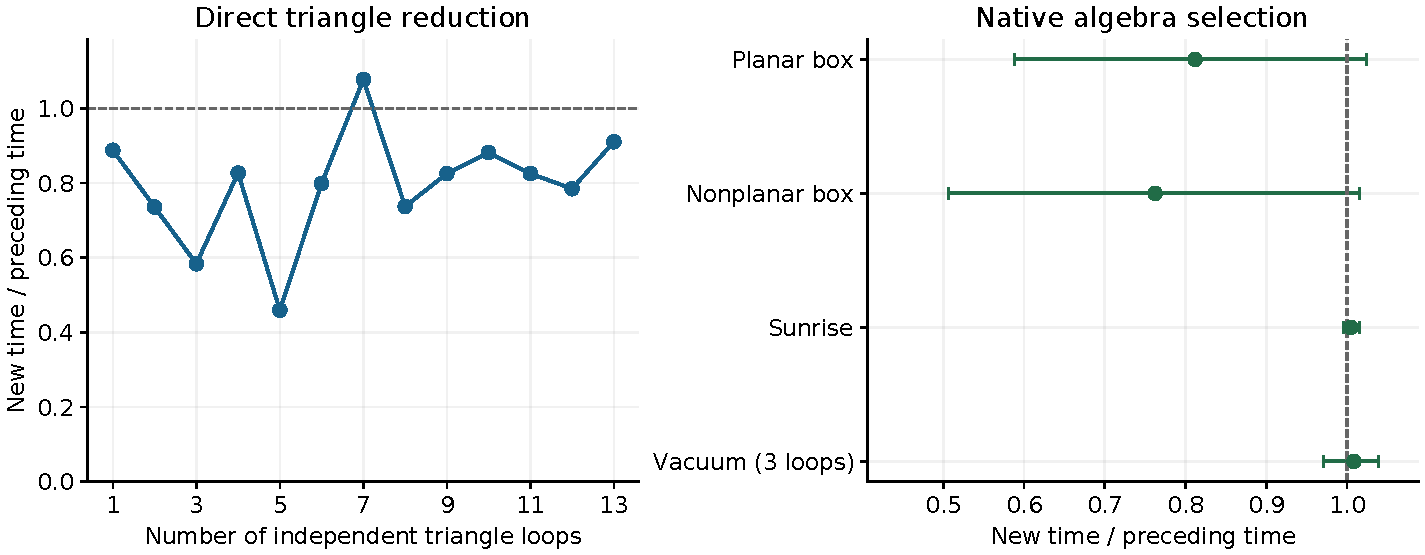
\includegraphics[width=\linewidth]{paper_figures/triangle_extension.pdf}
\caption{Complete-time ratios on the new requests. The dashed line marks equal time. The left panel shows the direct triangle implementation at each tested product loop order. The right panel shows native requests by propagator structure, with paired request-bootstrap intervals. Product tests do not establish connected higher-loop scattering performance.}
\label{notes-triangle:fig:triangle-extension}
\end{figure}

We also compare shared calls containing these 40 requests and the 53 preceding analytic regression requests. This preserves the setup benefit of the previously deployed method. Three complete repetitions use alternating method order and reverse the request order in the middle repetition. Two workers share an Intel Gold compute node, with one computation thread per application. The collection timer includes loading, all reductions, output reading, and cleanup.
\begin{table}[htbp]\centering\small
\caption{Shared-call time for the matched collection of 93 requests. The interval is the observed range of three complete repetitions, not a confidence interval.}
\label{notes-triangle:tab:triangle-batch}
\begin{tabular}{lrr}\toprule
Method & Median (s) & Observed range (s)\\\midrule
Preceding application & 46.642 & 46.337--48.713 \\
New fixed control & 40.561 & 39.524--46.243 \\
New integrated method & 40.696 & 40.194--41.472 \\
\bottomrule\end{tabular}\end{table}

The new-to-preceding collection ratio is 0.873. All 1,250 tested application results pass 19,946 exact coefficient comparisons after the stated basis conversion. The timed native procedures record 7 unsuccessful internal attempts across the fresh-call and shared-call comparisons; their recovery costs remain inside the timers. The separate formula checks add 120 high-precision Gamma-function comparisons, 4 exact index-shift checks, and 77 product checks. Native one-loop comparisons and the derivation support the triangle identity; the product tests check its separated-loop implementation.

\subsection{Final complete-call comparison}
A native reduction removes temporary files while it runs. The earlier resource monitor could stop a reduction if a directory disappeared during its inspection. We change the monitor to tolerate removal while preserving its storage bound. A controlled check reproduces the old exception and verifies the new behavior. This change affects runtime supervision and leaves the algebra and learned decisions unchanged.

We compare the preceding published application, the new mathematical method with the original monitor, and the final application with the corrected monitor on the same 93 requests. Each method runs three times on the same compute node with one worker, rotating method order, and reversed request order in the middle repetition. A preceding two-worker comparison showed timing differences larger than the measured monitor cost. It also stopped when recovery in the preceding application returned a 20-integral basis instead of the 16-integral reference basis for one vacuum request. We retain that failed comparison separately. The complete serial check uses every planned request and method. The complete timer includes unsuccessful internal attempts and recovery. Independent comparisons check the saved exact coefficients outside the timer.
\begin{table}[htbp]\centering\small
\caption{Final matched shared-call comparison. Times are complete collection times. The range shows the three observations. Internal failures count attempts across all three repetitions.}
\label{notes-triangle:tab:triangle-final}
\begin{tabular}{lrrrr}\toprule
Method & Median (s) & Mean (s) & Range (s) & Failures\\\midrule
Preceding application & 45.091 & 45.230 & 44.783--45.817 & 0 \\
New method, original monitor & 42.932 & 42.624 & 40.351--44.589 & 0 \\
Final application & 41.137 & 41.029 & 40.723--41.227 & 0 \\
\bottomrule\end{tabular}\end{table}
The final-to-preceding median ratio is 0.912, which reduces time by 8.8 percent on this collection. The final-to-original-monitor ratio is 0.958. All 837 application results pass 13,401 exact coefficient comparisons. This finite timing comparison does not prove a universal speedup or a globally shortest reduction.

The preceding parallel monitor comparison used two workers and stopped at the third published-application collection after the vacuum basis mismatch. Its recorded outputs pass 650 of 651 request comparisons. Its two complete matched repetitions give a final-to-published ratio of 0.847, and a corrected-to-original-monitor ratio of 1.131. The controlled serial repetition retains every physical input and algorithm. It changes the worker schedule to examine the unexplained timing difference. These two comparisons are reported separately.

\subsection{Verification imports}
Two verification helpers initially imported historical modules with the same names. We corrected these imports without changing the application, fitted model, or physical test inputs. We retained the completed timings and rechecked the saved results. The runtime-monitor comparison uses the corrected checks.

\subsection{Preparation checks and conservative admission}
The first native collection stopped at the three-loop vacuum request with squared masses $(1,1,1,13,13,64269)$. A probe batch size of eight disagreed with the preceding reference in the coefficient comparator. The collector stopped before it saved that candidate output, so its original difference cannot be reconstructed from the surviving record. The reference and failure log remain available. We corrected the collector to save a failed output before stopping.

Independent reruns compared symbolic algebra and several reconstruction settings. The original reference agreed with the symbolic result. Additional repetitions checked the disputed setting at four nearby mass profiles. These diagnostics did not justify treating the original failed check as a measured speedup. The new cost selector therefore retains the preceding application for this three-loop structure. The reserved comparison tests that conservative configuration. Independent symbolic reductions also check every action record used for fitting and validation.
